\section{Experiments}
\label{sec:experiments}

\subsection{Data}
\label{sec:data}


{\flushleft {\bf Questions:}} We assembled a corpus of 1,000 third to fifth grade standardized elementary school science exam questions, consisting of 346 publicly available questions gathered from standardized exams in 12 states, as well as 654 closed questions from an exam generating service. 
All questions are multiple choice with four possible answer candidates. Questions vary in length from 1 to 6 sentences, while the four multiple choice answer candidates are generally either single words or short phrases. 
Because of the small size of this corpus, our models were evaluated using 5-fold crossvalidation, with 3 folds for training, one for development, and one for test. 

{\flushleft {\bf Knowledge bases:}} Sentences from six text resources served as input for TAG generation.  Five of these resources are in the science domain and include two state-specific science exam study guides, a teacher's manual, a children's science dictionary, and a set of exam review flashcards.  Each of these in-domain resources was selected to be at a third-to-fifth grade knowledge level, and contained between 283 and 1,314 sentences (for a total of 3,832 in-domain sentences).  
The Simple Wiktionary\footnote{\url{http://simple.wiktionary.org}} was included as a large open-domain dictionary resource written at knowledge level similar to that of the exam questions.  Starting with over 24,000 definitions, we filtered these to include only definitions for nouns, verbs, and adjectives, for a total of 17,473 sentences after filtering.

\subsection{Tuning}
\label{sec:tuning}
We tuned the following hyperparameters once on the development data to optimize both performance and stability.

{\flushleft \textbf{Number of candidate justifications:}} 
Each of the multiple choice answers can have a large number of candidate justifications.  To reduce runtime and assist learning, we filter this initial list of TAGs to include only a subset of TAGs with a high focus word mass. We kept all justifications tied for focus mass with the justification in 25th place, resulting in a variable number of TAGs for each QA pair.  For our dataset, the mean number of TAGs for each QA pair was 141. \\

{\flushleft \textbf{Perceptron Hyperparameters:}} We investigated the perceptron hyperparameters using a coarse grid search and found a stable optimum with 10 epochs, a $\tau$ of 1.0, burn in of 5 epochs (i.e., the weight updates were not added to the average weights for the first five epochs), and a learning rate (which dampened the updates to the weight vector) of 0.1. Since model results can vary depending on the random seed used for initialization, rather than using a single perceptron we use an ensemble of 50 perceptron models initialized with random weights.  These models are combined in a simple voting scheme, where each model casts a single vote for each question (distributing the vote only in the case of ties).\\

{\flushleft \textbf{Feature Normalization:}} To minimize the effect of outliers in the feature space, we log-transformed the feature values, and then rescaled each feature independently to lie within the range of $-1$ to $1$, using the formula
\mbox{$normalized  = lower + (original - min)\frac{(upper - lower)}{(max - min)}$},
where $upper$ and $lower$ are the desired boundaries for the normalization ($1$ and $-1$, respectively), $max$ and $min$ are the maximum and minimum values for the corresponding feature across the training dataset, and $normalized$ is the result of normalizing $original$.
Note that during testing it is possible to see feature values outside of their known $[min, max]$ interval, which means that after normalization their values will fall outside the $[-1, 1]$ interval. We do not do any additional post-processing for these values.


\subsection{Baselines}
\label{sec:baselines}

We include the following baselines: 

{\flushleft {\bf Random:}} selects an answer randomly.
{\flushleft {\bf Candidate retrieval (CR):}} ranks answers using an approach similar to the baseline model in Jansen et al.~\citeyear{jansen14}, which uses features that measure cosine similarity over {\em tf-idf} vectors (e.g., Ch. 6, Manning et al.\citeyear{manning08}) to rank answer candidates in a ``learning to rank'' (L2R) framework.  
Traditionally, with retrieval systems, short answers to questions are dynamically constructed from larger parent documents, and the top-scoring answer (defined as the answer with the highest {\em tf-idf} score between that answer candidate and a query vector made from the question) is taken to be the winner.  Here we adapt this setup to multiple choice exams by: (a) using query vectors that contain words from both the question and multiple choice answer candidate, and (b) generating features from the top {\em tf-idf} score for each answer candidate in a given question, which are then combined in the learning-to-rank framework.  We then take the short passage retrieved by the system as a justification for why that answer candidate is correct. 

Documents are constructed across the six knowledge bases by dividing each corpus by subsection (for texts), by definition (for dictionaries), or by flashcard.  We implemented the document indexing and retrieval system using Lucene\footnote{\url{http://lucene.apache.org}}.  Each sliding window of $N$ sentences in a given document served as a potential answer justification. Using the development questions, we empirically determined that a two-sentence window performed best, though performance did not significantly differ for window sizes between one and five sentences.  This  model generates two features: a cosine similarity score between the query vector and the best-scoring candidate answer justification in a given corpus, and a linear model that combines this cosine similarity with the cosine similarity between the query vector and the entire document, blending both local (answer justification) and global (document) context. 

Because our six corpora are of different genres (study guide, teachers guide, dictionary, flashcards), domains (science-domain vs. open-domain), and lengths (300 to 17,000 sentences), we implement six separate {\em tf-idf} models, each containing documents only from a single corpus. We then combine the two retrieval features from each model (12 features total) into a ranking perceptron \cite{Shen:Joshi:2005,Surdeanu:11} to learn which knowledge bases are most useful for this task.  This ensemble retrieval model produces a single score for each multiple choice answer candidate, where the top-scoring answer candidate is selected as the winner.  The top-scoring answer justifications from each of the six retrieval models then serve as justifications. 


 
{\flushleft {\bf Jansen et al. (2014):}} the best-performing combined lexical semantic (LS) and CR model of Jansen et. al~\citeyear{jansen14}, which was shown to perform well for open domain questions.  Similar to the CR model, we adapted this model to our task by including six separate recurrent neural network language models (RNNLM) of Mikolov et al.\citeyear{mikolov13,mikolov10}, each trained on one of the six knowledge bases.  Two features that measure the overall and pairwise cosine similarity between a question vector and multiple choice answer candidate vector are included.  The overall similarity is taken to be the cosine similarity of the composite vectors of both the question and answer candidate, obtained by summing the vectors for the individual words within either the question or answer candidate vectors, then renormalizing these composite vectors to unit length.  The pairwise similarity is computed as the average pairwise cosine similarity between each word in the question and answer candidate.  Two features from each of the six LS models are then combined with the two features from each of the CR models (24 features total) as above using a ranking perceptron, with the top-scoring answer candidate taken as correct.  Because the LS features do not easily lend themselves to constructing answer justifications, no additional human-readable justifications were provided by this model. 


\subsection{Results}
\label{sec:results}

Here we first investigate the performance of two variants of the TAG model with respect to justification length.  We then compare the best-performing model with the baselines, and show that the TAG and CR models can be combined to increase performance. We use the standard implementation for precision at 1 (P@1) ~\cite{manning08} and a tie-aware implementation of mean reciprocal rank (MRR) \cite{mcsherry2008}.



%
% Performance versus path length
%
\begin{table}[t]
\caption{{
Performance as a function of justification length in sentences (or, the number of graphlets in a TAG) for two models: one aware of connection-type, and one that is not. Bold font indicates the best score in a given column for each model group. 
}}
\small
\begin{center}
%\begin{tabular}{p{0.3mm}p{55mm}llll}
\begin{tabular}{lllll}
\multicolumn{1}{l}{ } & \multicolumn{1}{l}{ } & \multicolumn{1}{l}{P@1} & \multicolumn{1}{l}{ } & \multicolumn{1}{l}{MRR} \\
\multicolumn{1}{l}{ Model } & \multicolumn{1}{l}{P@1} & \multicolumn{1}{l}{Impr.} & \multicolumn{1}{l}{MRR} & \multicolumn{1}{l}{Impr.} \\
\hline
\multicolumn{5}{l}{Normal}\\
\hline
1G					& 35.33			& --				& 59.26  		&	--  \\
2G					& {\bf 38.16}	& {\bf 8.0\%}	& {\bf 61.33}  	&	{\bf 3.5\%}  \\
3G					& 37.78			& 6.3\%			& 61.14  		&	3.2\%  \\
\\
\hline
\multicolumn{5}{l}{Connection-type aware (Daum{\'e})}\\
\hline
1G\textsubscript{CT}			& 34.80			& --				& 58.86  		& --  \\
2G\textsubscript{CT}			& {\bf 39.91}	& {\bf 14.7\%}	& {\bf 62.53}  	& {\bf 6.2\%} \\
3G\textsubscript{CT}			& 38.53			& 10.7\%			& 61.65  		& 4.7\%  \\

\hline
\end{tabular}

%space{-6mm}
\label{tab:pathlength}
\end{center}
\end{table}


\subsubsection{Justification Length}
\label{sec:pathlength}
Table~\ref{tab:pathlength} shows the performance of the TAG model as a function of increasing justification length.
Here, the $k$G models contain exclusively justifications of length $k$ (we explore TAGs of varying length later in this section).
Short two-sentence (or two-graphlet) TAGs significantly outperform single sentence TAGs, with single sentence (1G) TAGs starting at 35.3\% P@1, increasing to 38.2\% for two-sentence (2G) TAGs, hen decreasing slightly to 37.8\% for three-sentence (3G) TAGs. 
In previous work, we observed that for a variety of word-level graphs and traversal algorithms, QA performance tends to rapidly peak when aggregating two or three words, then slowly decreases as more words are aggregated due to ``inference drift'' in the graph 
traversal process
(i.e., following the connections from \emph{breakfast} $\rightarrow$ \emph{hashbrowns} $\rightarrow$ \emph{potato} $\rightarrow$ \emph{field} would potentially connect questions about breakfast to information about potato or even soccer fields)   \cite{fried2015higher}.  

Though our sentence aggregation model contains far more structure than the higher-order lexical semantic graphs of Fried et al. ~\citeyear{fried2015higher}, and is represented at the level of the sentence or graphlet rather than individual lemmas, we hypothesize based on this previous work that we may be observing the beginning of same characteristic peak in performance reported there.  Because runtime increases exponentially with the number of sentences included in a TAG, it quickly becomes intractable to test this with TAGs containing more than 3 graphlets. 

Extending the model to include a knowledge of the connection type (or the type of lexical overlap, see Section~{\ref{sec:characterizing}) between sentences in a given TAG using Daum{\'e}'s method~\cite{daume2007} increases performance, suggesting that different kinds of connections are best identified through different feature patterns.  Here, the connection-type aware 2G\textsubscript{CT} model outperforms the regular 2G model by nearly 2\% P@1 (absolute), increasing performance to 39.9\% -- an increase of +14.7\% (relative) over using only single-sentence TAGs.\footnote{Each of the 50 models in the ensemble reranker is initialized with random weights, causing the small performance difference between 1G and 1G\textsubscript{CT}}





\subsubsection{Combined Models}
\label{sec:combinedmodels}
%
% Combined model performance
%
\begin{table*}[t]
    \small
    \caption{{
Performance of the baseline and best-performing TAG models, both separately and in combination. TAG justifications of different short lengths were found to best combine in single classifiers (denoted with a $+$), where models that combine the CR baseline or long (3G) TAG justifications best combined using voting ensembles (denoted with a $\cup$). Bold font indicates the best score in a given column for each model group. Asterisks indicate that a score is significantly better than the highest-performing baseline model (* signifies $p < 0.05$, ** signifies $p < 0.01$).  The dagger indicates that a score is significantly higher than the score in the line number indicated in superscript ($p < 0.01$). All significance tests were implemented using one-tailed non-parametric bootstrap resampling using 10,000 iterations. }}
\begin{center}
\begin{tabular}{p{0.3mm}p{55mm}llll}
\multicolumn{1}{l}{ } & \multicolumn{1}{l}{ } & \multicolumn{1}{l}{ } & \multicolumn{1}{l}{P@1} & \multicolumn{1}{l}{ } & \multicolumn{1}{l}{MRR} \\
\multicolumn{1}{l}{\#} & \multicolumn{1}{l}{ Model } & \multicolumn{1}{l}{P@1} & \multicolumn{1}{l}{Impr.} & \multicolumn{1}{l}{MRR} & \multicolumn{1}{l}{Impr.} \\

\hline
& \multicolumn{5}{l}{Baselines }\\
\hline
1 & Random					& 25.00 			& --		& 52.08  		& --	  \\
2 & CR 						& {\bf 40.20} 	& -- 	& {\bf 62.49}	&	--  \\
3 & Jansen et al. (2014)		& 37.30 			& --		& 60.95 			& 	--	 \\

\\
\hline
& \multicolumn{5}{l}{Combined models with justifications of variable lengths (Single classifier)}\\
\hline
4 & 1G + 2G										& 38.69			& --		& 61.43  	& --  \\
5 & 1G\textsubscript{CT} + 2G\textsubscript{CT} 	& {\bf 42.88$\dagger ^4$}	& {\bf +6.7\%}		& {\bf 63.94\%}  	& {\bf +2.3\%}	  \\

\\
\hline
& \multicolumn{5}{l}{Combined models that include the CR baseline (Voting)}\\
\hline
6 & CR $\cup$ 1G\textsubscript{CT} $\cup$ 2G\textsubscript{CT} $\cup$ 3G\textsubscript{CT} 			& 43.15*			& +7.3\%			& 64.51*		& +3.2\%	  \\
7 & CR $\cup$ (1G\textsubscript{CT} + 2G\textsubscript{CT}) $\cup$ 3G\textsubscript{CT} 			& {\bf 44.46**}		& {\bf +10.6\%}		& {\bf 65.53**} 		& {\bf +4.9\%}	  \\

\hline
\end{tabular}
%space{-6mm}
\label{tab:combinedmodels}
\end{center}
\end{table*}

Where Table~\ref{tab:pathlength} lists models that contain justifications of static length, Fried et al.~\citeyear{fried2015higher} showed that combining paths of different lengths into a single classifier can increase performance.  The performance of TAG models that combine justifications of different lengths, as well as the baseline models, is shown in Table~\ref{tab:combinedmodels}.

{\flushleft {\bf Baselines:}} Where the lexical semantics model of Jansen et al. ~\citeyear{jansen14} outperformed their CR baseline by +36\% (relative) on a large corpus of open-domain questions from Yahoo Answers, here on elementary science exams, the lexical semantic features decrease performance.  Our conjecture is that the performance difference is due to the difference in the size of the corpora used to train the lexical semantic model -- where Jansen et al. trained their lexical semantic model using Gigaword, here we are limited by the relatively small size of our text resources.  Jansen et al. ~\citeyear{jansen14} reported that a domain-specific version of their lexical semantic model performed poorly when trained on a biology textbook and subset of Wikipedia, and others have since shown that lexical semantic models perform poorly with small amounts of training data \cite{sharp-EtAl:2015:NAACL-HLT}. 

{\flushleft {\bf Combined Models:}} Single-classifier models containing both 1G and 2G TAGs were generated for both the normal and connection-type-aware models.  The 1G + 2G model performs only slightly better than 2G alone, but when the models are connection-type aware, there is greater benefit to combining the different path lengths -- the connection-type-aware 1G\textsubscript{CT} + 2G\textsubscript{CT} model (line 5) increases performance to 42.9\% P@1 (compare to the static-length 2G\textsubscript{CT} performance of 39.9\%).


As the CR baseline and the TAG models are performing inherently different tasks (information \emph{retrieval} and information \emph{aggregation} respectively), we are able to combine them together in a voting model in order to create a full system that contains the benefits of each.
The voting models that incorporate both the CR baseline and TAG models across all justification lengths are included on lines 6 and 7.  Both models significantly increase performance over the CR baseline, with the voting model that couples 1G\textsubscript{CT} + 2G\textsubscript{CT} as a single classifier (and single vote) performing better than when 1G\textsubscript{CT} and 2G\textsubscript{CT} vote separately.  This best-performing model reaches 44.5\% P@1, increasing performance over the CR baseline by +10.6\% (relative). %All in all
This set of experiments demonstrates that our approach of jointly ranking answers and justifications is complementary to a strong information retrieval baseline, and significantly improves performance at the task of selecting the correct answer.  


\subsubsection{Justifications}


%
% Justification example (IR)
%
\begin{table*}[t]
\caption{{ \label{font-table} Example justifications from the CR baseline and their associated ratings. }} %  (N=20, c=0.1)
\begin{center}
\begin{footnotesize}
%\begin{tabular}{lcc}
%\cline{2-3}
%\begin{tabular}{cl}
\begin{tabularx}{\textwidth}{p{1cm}p{11.5cm}}
%\multicolumn{1}{r}{} & \multicolumn{1}{l}{} \\
%\cline{1-2}
%\hline
\hline
\multicolumn{1}{c}{} & \multicolumn{1}{c}{Question} \\
\hline			
\multicolumn{2}{l}{	What is the interaction between the producer and the consumer in a food chain?} \\
		&	\textbf{[A] The consumer eats the producer for energy.}  \\
		&  [B] The consumer does not interact directly with the producer. \\
			&   [C] The producer eats other producers for energy.   \\
			& [D] The producer eats the consumer for energy. \\
%Answer		&	The consumer eats the producer for energy. \\			

\multicolumn{1}{c}{} & \multicolumn{1}{c}{} \\				
\hline
\multicolumn{1}{l}{Rating} & \multicolumn{1}{c}{Example Justification} \\
\hline			
{\em Good }		&	A primary (1st) consumer eats producers (plants). A secondary (2nd) consumer eats primary consumers. {\em [Barrons SG]}  	\\
{\em Half }		&	The food chain starts with a producer (a plant) and ends with a decomposer. {\em [Flashcards]} \\
{\em Topical }	&   A herbivore is an organism that depends on plants for most of its food and energy. {\em [Science Dictionary]} \\
{\em Offtopic }	&	When a plate moves suddenly a great amount of energy is released.  These waves cause damage...  {\em [Virginia SG]} \\
%\end{tabular}
\end{tabularx}
\end{footnotesize}
\label{tab:justificationsIRexamples}

\end{center}
\end{table*}


%
% Justification example (TAG)
%
%\begin{figure}[t!]
%\begin{center}
%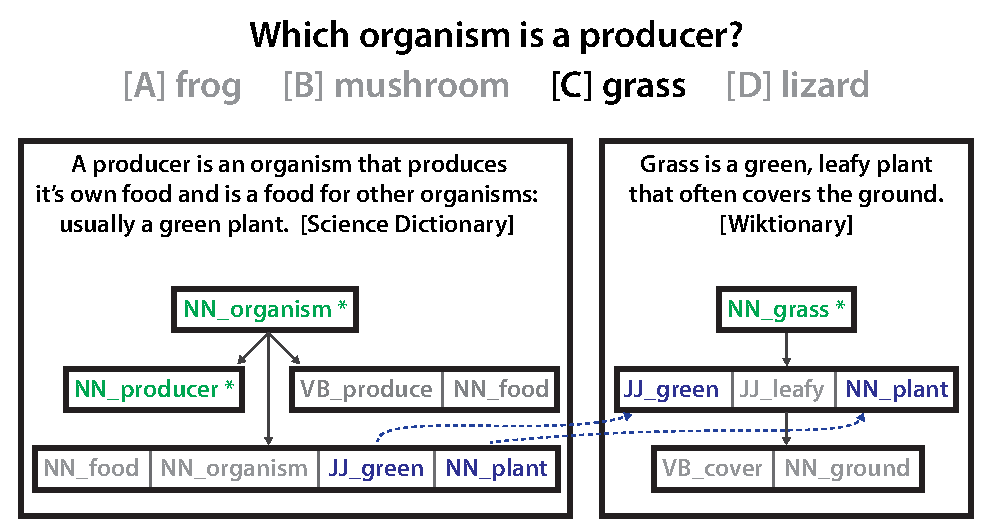
\includegraphics[width=75mm]{example_tig_producer2.pdf}
%\vspace{-2mm}
%\caption{ An example TAG path and justification rated as {\em good}. \note{TODO: Redraw figure with different line widths, closer to the original DOT file?}}
%%\caption{{\small An example of the alignments produced by the two discourse models.  The sequential model aligns pairs of consecutive sentences, capturing intersentence associations such as \emph{cider--apples}, and \emph{orchard--autumn}.  The RST model generates alignment pairs from participants in all (binary) discourse relations, capturing both intrasentence and intersentence alignments, including 
%%\emph{apples--orchard, cider--apples}, and \emph{cider--autumn}.}}
%% ms: I get the point, but there is value in brevity. Plus, maybe we should not use Bob as example :)
%%the intersentence alignments above along with intrasentence and multi-sentence alignments, including \emph{Bob--cider, apples--orchard}, and \emph{cider--autumn}.}}
%\vspace{-5mm}
%\label{fig:justificationTAGexample}
%\end{center}
%\end{figure}



\begin{table}[]
\small
\caption{{An example TAG and justification rated as {\em good}.  The two sentences connect on non-focus "other" shared words (e.g., \emph{green, plant}) which are not found in the question or answer, but which are highly related to the focus words. }} 
\begin{tabularx}{\textwidth}{p{2.5cm}p{11cm}}
%\hline
%\multicolumn{2}{l}{EXAMPLE: Other} \\
\hline
% Question Info
Question & Which organism is a producer? (GR:5)     \\
Focus Word(s) &   (NN\_producer, 0.92) (NN\_organism, 0.08) \\
Answers & (A) frog  (B) mushroom   (C) grass    (D) lizard \\
\hline
% Correct Answer Info
Correct Answer &  grass \\
Focus Word(s) &   (NN\_grass, 1.00) \\
\multicolumn{2}{c}{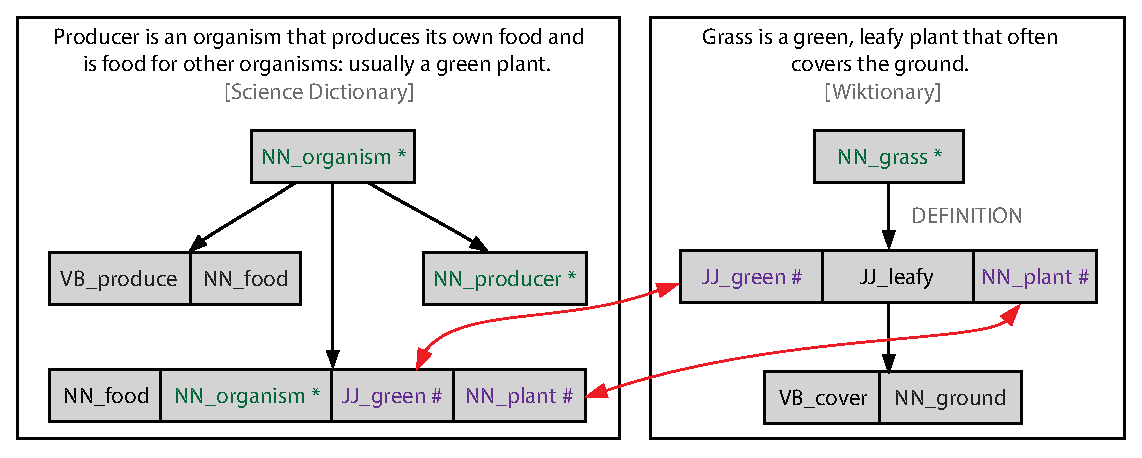
\includegraphics[width=115mm]{tag_good_justification.pdf}}
\\
\hline
\end{tabularx}
\label{ex:tagQsXs}
\end{table}






%
% Justification Examples - EXTRA
%
%\begin{table}[]
%\caption{{  Example of a TAG {\bf connected on answer focus} words. }} 
%\begin{tabularx}{\textwidth}{p{2.5cm}p{11cm}}
%%\hline
%%\multicolumn{2}{l}{EXAMPLE: Other} \\
%\hline
%% Question Info
%Question & What are the stages of development of an organism called? (GR:5)   \\
%Focus Word(s) &  (NN\_organism, 0.80) (NN\_stage, 0.13) (NN\_development, 0.07) \\
%\hline
%% Correct Answer Info
%Correct Answer &  Life cycle \\
%Focus Word(s) &  (NN\_cycle, 0.92) (NN\_life, 0.08) \\
%\multicolumn{2}{c}{\includegraphics[scale=0.5]{q58a1p2363connection.png}}\\
%\hline
%\end{tabularx}
%\label{ex:tagAns}
%\end{table}

%\begin{table}[]
%\caption{{  Example of a TAG {\bf connected on question and answer focus words}. (Somewhat more challenging focus word extraction, but we end up matching most of the words).  }} 
%\begin{tabularx}{\textwidth}{p{2.5cm}p{11cm}}
%%\hline
%%\multicolumn{2}{l}{EXAMPLE: Other} \\
%\hline
%% Question Info
%Question & Different types of organs that work together to perform a specific life function are called a(n) \_\_\_. (GR:5)   \\
%Focus Word(s) &   (VB\_work, 0.23) (VB\_perform, 0.23) (NN\_n, 0.23) (RB\_together, 0.09) (NN\_life, 0.07) (JJ\_specific, 0.06) (JJ\_different, 0.04) (NN\_function, 0.03) (NN\_organ, 0.01) \\
%\hline
%% Correct Answer Info
%Correct Answer &  organ system \\
%Focus Word(s) &   (NN\_system, 0.67) (NN\_organ, 0.33) \\
%\multicolumn{2}{c}{\includegraphics[scale=0.5]{q61a2p1104connection.png}}\\
%\hline
%\end{tabularx}
%\label{ex:tagQuest+Ans}
%\end{table}

%\begin{table}[]
%\caption{{  Example of a TAG connected only on answer focus words. Despite a non-ideal ranking of the question focus words, the system is able to lock onto this as a good justification of the correct answer.}} 
%\begin{tabularx}{\textwidth}{p{2.5cm}p{11cm}}
%%\hline
%%\multicolumn{2}{l}{EXAMPLE: Other} \\
%\hline
%% Question Info
%Question & Pots and pans are most often made from metal because \_\_\_. (GR:5)     \\
%Focus Word(s) &   (NN\_pot, 0.48) (NN\_pan, 0.48) (NN\_metal, 0.04) \\
%\hline
%% Correct Answer Info
%Correct Answer &  metals conduct heat well \\
%Focus Word(s) &   (NN\_heat, 0.44) (RB\_well, 0.44) (NN\_metal, 0.07) (VB\_conduct, 0.04) \\
%\multicolumn{2}{c}{\includegraphics[scale=0.5]{q100a3p908connection.png}}\\
%\hline
%\end{tabularx}
%\label{ex:tagXs}
%\end{table}

%\begin{table}[]
%\caption{{  {\bf Error example: Construction and Ranking vs Answer Selection:} Example of a question which requires {\bf complex inference}.  Our system aggregate sentences by connecting on {\bf question focus words as well as non-focus words}, to construct a good justification for the correct answer and rank it to the top of the justifications for that answer candidate. }} 
%\begin{tabularx}{\textwidth}{p{2.5cm}p{11cm}}
%%\hline
%%\multicolumn{2}{l}{EXAMPLE: Other} \\
%\hline
%% Question Info
%Question & In a food chain or web, the most efficient users of the Sun's energy are \_\_\_. (GR:5)     \\
%Focus Word(s) &   (NN\_chain, 0.23) (NN\_web, 0.23) (NN\_user, 0.22) (NN\_energy, 0.22) (NN\_food, 0.05) (NN\_sun, 0.03) (JJ\_efficient, 0.02) \\
%\hline
%% Correct Answer Info
%Correct Answer &  herbivores \\
%Focus Word(s) &   (NN\_herbivore, 1.00) \\
%\multicolumn{2}{c}{\includegraphics[scale=0.5]{q67a2p1connection.png}}\\
%\hline
%\end{tabularx}
%\label{ex:tagQsXsWrong}
%\end{table}
%
%
%\begin{table}[]
%\caption{{  {\bf Error example:} A similar example to the last one -- much of the time we're able to construct and rank very good TAGs (for a given answer candidate), but the last step -- selecting the best justification, is more sensitive to {\emph well connected answers} rather than {\emph good answers}.  Here the two aggregated sentences are {\bf connected on question focus words.}  }} 
%\begin{tabularx}{\textwidth}{p{2.5cm}p{11cm}}
%%\hline
%%\multicolumn{2}{l}{EXAMPLE: Other} \\
%\hline
%% Question Info
%Question & All organisms need food to survive. Which statement best describes the purpose of food for organisms? (GR:4)    \\
%Focus Word(s) &   (NN\_organism, 0.34) (NN\_organism, 0.34) (VB\_survive, 0.08) (NN\_food, 0.05) (VB\_need, 0.03) (NN\_food, 0.08) (NN\_purpose, 0.05) (NN\_statement, 0.03) \\
%\hline
%% Correct Answer Info
%Correct Answer &  Food provides energy for growth. \\
%Focus Word(s) &   (NN\_energy, 0.68) (NN\_growth, 0.16) (VB\_provide, 0.11) (NN\_food, 0.05) \\
%\multicolumn{2}{c}{\includegraphics[scale=0.5]{q19a3p2833connection.png}}\\
%\hline
%\end{tabularx}
%\label{ex:tagQsAsWrong}
%\end{table}
%
%
%
%\begin{table}[]
%\caption{{ {\bf Error example:} Another example of {\bf complex inference} that {\bf connects on other words}, in this case {\emph river}.  Again we're ranking this \todo{path} to the candidates for a given answer, but not selecting it out of the 4 multiple choice answers.  }} 
%\begin{tabularx}{\textwidth}{p{2.5cm}p{11cm}}
%%\hline
%%\multicolumn{2}{l}{EXAMPLE: Other} \\
%\hline
%% Question Info
%Question & Moving water was the most important factor in forming which of these? (GR:5)   \\
%Focus Word(s) &   (VB\_move, 0.68) (NN\_factor, 0.16) (NN\_water, 0.11) (JJ\_important, 0.05) \\
%\hline
%% Correct Answer Info
%Correct Answer &  the Grand Canyon \\
%Focus Word(s) &   (NN\_canyon, 0.67) (NN\_grand, 0.33) \\
%\multicolumn{2}{c}{\includegraphics[scale=0.5]{q33a0p57connection.png}}\\
%\hline
%\end{tabularx}
%\label{ex:tagXsWrong}
%\end{table}

The previous experiments demonstrate that our method performs well at identifying correct answers. But how well does it perform at the task of {\em justifying} those answers?
We evaluated justification performance for both the best baseline (CR) and the best performing TAG model that is independent of CR (i.e., 1G\textsubscript{CT} + 2G\textsubscript{CT}) .  Where TAG justifications took the form of the sentences being aggregated, justifications for the CR model were taken to be the highest-scoring short passages from each of the six knowledge bases.  As the CR model was tuned to a retrieval size of two sentences to maximize P@1 performance, each CR justification was two sentences in length.\footnote{Documents for the dictionary and flashcard corpora typically contained only a single sentence, and so answer justifications from these corpora are often shorter than two sentences.} To facilitate easy comparison, since the CR model provides six justifications (one from each knowledge base), we evaluate the top six scoring TAG justifications.  

The correctness of justifications was independently annotated by two of the authors. Any detected conflicts were resolved post hoc by the two annotators working together.
%
Answer justifications were rated on a four-point scale, based on their ability to provide a convincing justification to the user as to why a given answer choice was correct (see  Table~\ref{tab:justificationsIRexamples} for CR examples, and Figure~\ref{ex:tagQsXs} for a TAG example).   Justifications rated as {\em\bf good} describe the inference required to arrive at the correct answer.  Those rated as {\em\bf half} contained at least a portion of an explanation of the inference, but missed some critical aspect required to answer the question, like discussing producers but not consumers in Table~\ref{tab:justificationsIRexamples}. The two final ratings are for justifications that did not address the inference -- {\em\bf topical} justifications do not address the question but discuss a similar topic, where {\em\bf offtopic} justifications are unrelated to the question. 

%
% Justification performance
%
\begin{table}[t]
\small
\caption{{ \label{font-table} \emph{At least one} justification performance for both CR and TAG models, reflecting the highest rating attained by at least one of the top six justifications for a given question. }}%  Precision@6 performance reflects the overall proportion of each rating across all of the top six justifications. }} % 
\begin{center}
\begin{tabular}{p{20mm}cc}
\hline
\multicolumn{1}{l}{Rating} & \multicolumn{1}{c}{CR} & \multicolumn{1}{c}{TAG} \\%  & CR & TAG \\
\cline{2-3}
\hline
Good				&	45.3\%		& 56.7\%	 \\%	& 12.6\%		& 45.1\%	 \\
Half				&	34.9\%		& 20.7\%	 \\%	& 17.3\%		& 18.0\%	 \\
Topical			&	11.9\%		& 14.4\%	 \\%	& 17.2\%		& 18.4\% \\
Offtopic			&	7.9\%		& 8.2\%	 \\%	& 52.9\%		& 18.5\% \\

\end{tabular}
%\end{footnotesize}

 
\label{tab:justifications}

\end{center}
\end{table}

We evaluated the top-rated answer justifications using an {\bf at least one} method.  With this method, performance reflects the highest rating attained by \emph{at least one} of the six justifications for a given question. For example, for a question to be classed as {\em good}, at least one of the six answer justifications must be rated as {\em good}.  \emph{At least one} answer justification performance is listed in Table~\ref{tab:justifications}. For the TAG model, 56.7\% of the questions had at least one justification rated as {\em good}, outperforming CR justifications by 11.4\% (absolute).  


This experiment supports our original intuition that justifications must be aggregated from multiple resources. While the small window of sentences from the CR model is sufficient to justifiably answer many questions, a large number of questions require knowledge to be aggregated from {\em non-adjacent} sentences within a given corpus, or from sentences in different corpora altogether, to compose convincing answer justifications.  While the CR model leaves many of these questions with only partial justifications (34.9\% of justifications are rated as {\em half}), the TAG model  is able to aggregate sentences from multiple sources, and finds complete {\em good} justifications for many of the questions only partially answered by the CR model.


\subsubsection{Ablation Studies}
\label{sec:controls}
To verify the contribution of the components of our system, we include the following ablation studies:
%\paragraph{How does the latent layer in the Ranking Perceptron affect performance?}
{\flushleft {\bf Latent Perceptron:}} The complete removal of the latent layer (i.e., using the average of all TAG scores to score the candidate answer, and performing perceptron updates with all TAGs) decreases the performance of the best performing TAG model (1G\textsubscript{CT} + 2G\textsubscript{CT}) from 42.88 to 35.43 P@1.  Alternatively, we experimented with using the sum of the TAG scores and the maximum TAG score as the candidate score, while still doing updates with all TAGs.  These configurations decreased performance to 34.46 and 38.09 P@1, respectively. This demonstrates the importance of modeling justification quality as a latent variable.

%\paragraph{How do the focus words impact performance?}
{\flushleft {\bf Focus Words:}} Focus words are used both to find relevant sentences to aggregate into answer justifications, as well as to characterize those justifications when expressed as TAGs. Replacing focus words with uniform weights for all content words (NN, VB, JJ) in a question reduces performance of the 1G+2G model from 38.69 to 33.89 P@1.  For the connection-type-aware model (1G\textsubscript{CT} + 2G\textsubscript{CT}), performance decreases from 42.88 to 40.03 P@1. This supports our observation that science exam questions contain several layers of information (e.g., the underlying question, and the example the question is grounded in), each contributing different utility to the QA process. 

%\paragraph{How does the graphlet structure impact performance?}
{\flushleft {\bf Graphlet Structure:}}  Graphlets segment sentences based on clausal and prepositional boundaries to facilitate evaluating how well two sentences connect using structures larger than a word but more fine-grained than the entire sentence.  
In other words, graphlets are the key structure in our representation of answer justifications because they drive both intra- and intersentence connections in a TAG. 
Eliminating this structure (i.e., considering each sentence as a bag of words, which is equivalent to a graphlet with a single nugget)
substantially reduces the performance of the 1G + 2G model from 38.69 to 28.90 P@1 and the performance of the 1G\textsubscript{CT} + 2G\textsubscript{CT} model from 42.88 to 28.08 P@1. 

\begin{figure}
\centering
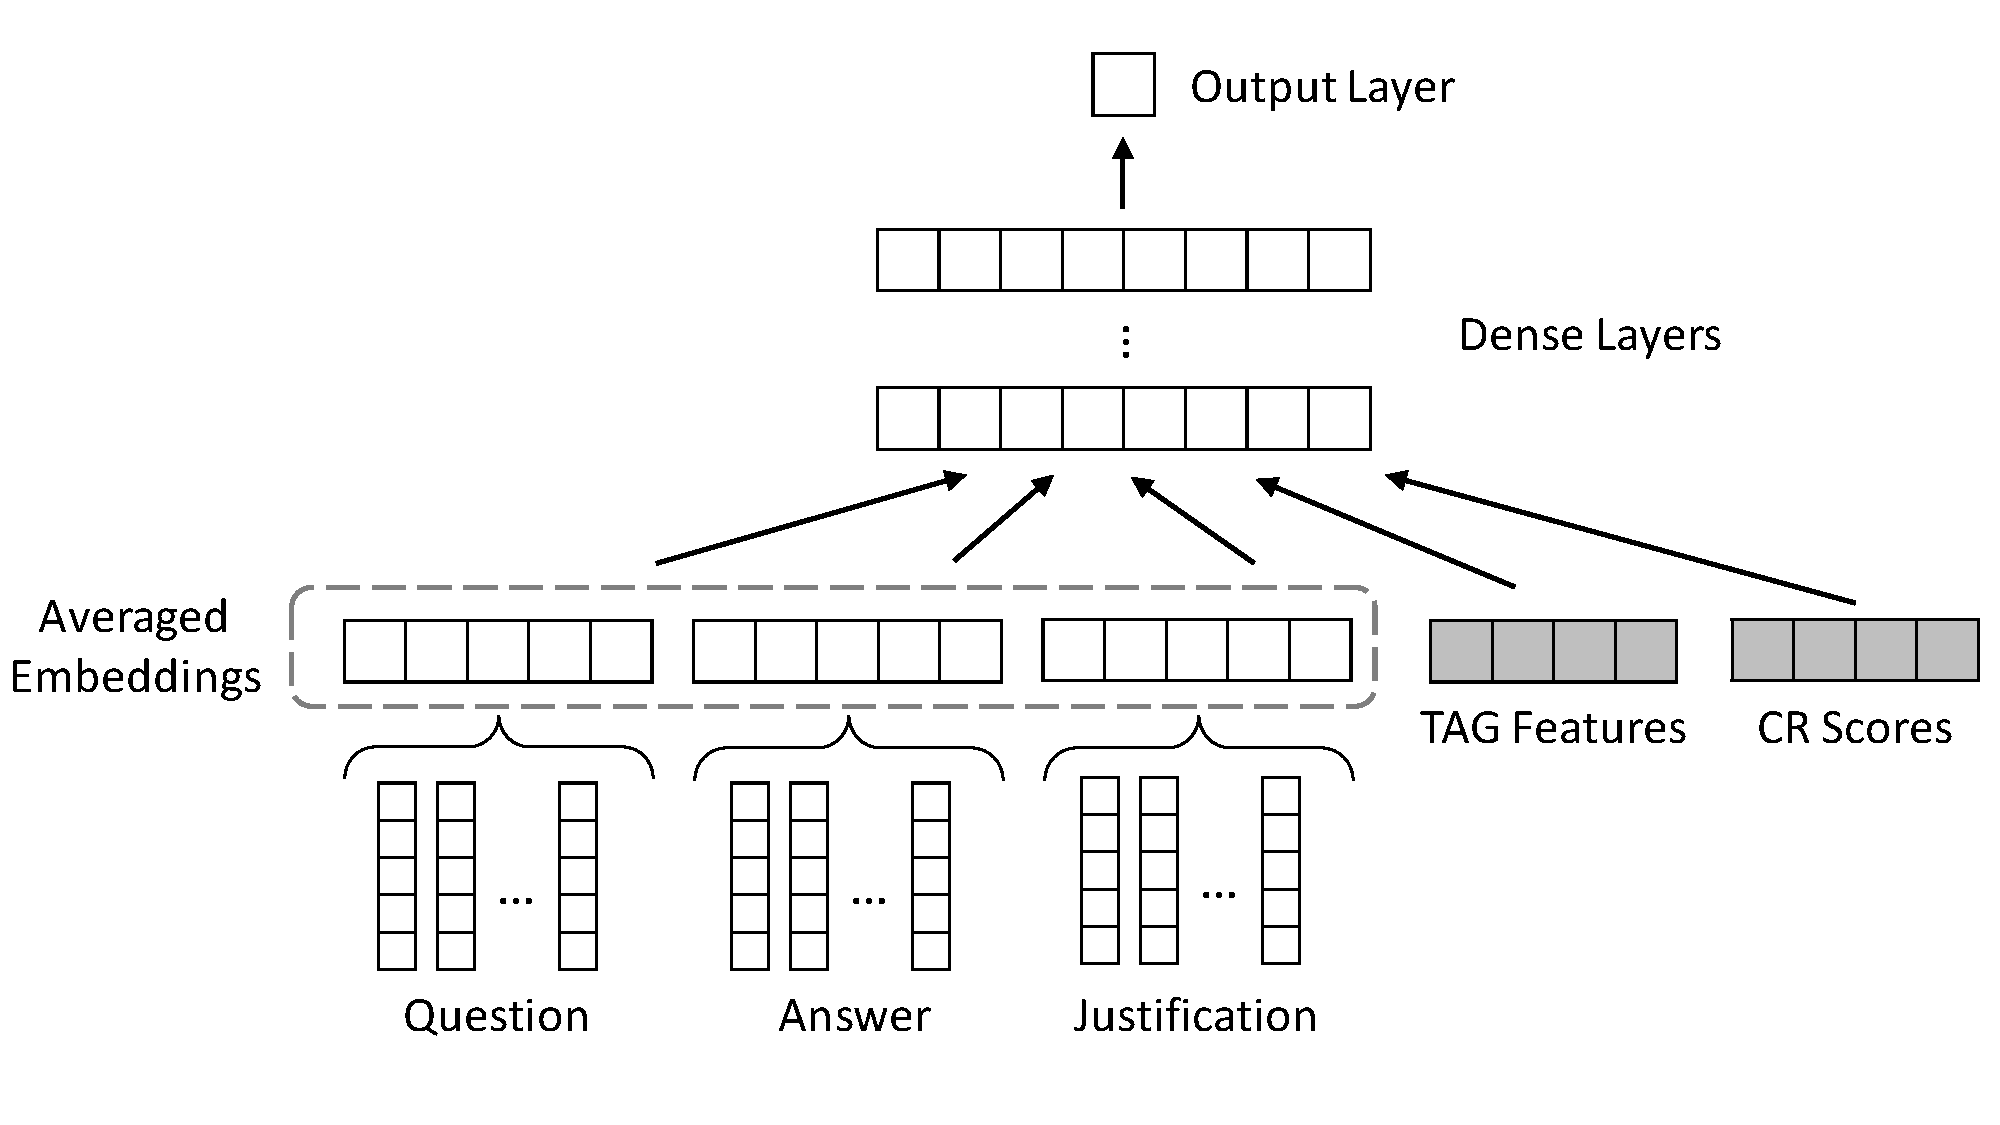
\includegraphics[width=0.8\textwidth]{tagNNArch2scores.pdf}
\caption{The architecture for the neural network variation of our TAG system. We use a fully-connected feed-forward network which takes as input the content words (i.e., nouns, verbs, and adjectives) from the question, candidate answer, and corresponding justification.  For each of these, we create a composite vector by averaging the embeddings of the individual words.  We then concatenate these three composite vectors, as well as the TAG features and the CR scores, to form the input layer to the network. The output of the network is a single, real-valued score for the candidate answer justification.}
\label{fig:nn_arch}
\end{figure}

\subsection{From Latent Perceptron to Latent Neural Networks}
\label{sec:nn}

Neural networks (NNs) have recently received much attention in many NLP tasks and have been shown to be quite effective in certain question answering tasks~\cite{Iyyer2014,bordes2014question,bordes2015large,Iyyer2015,wang2015long,dong2015question,yih2015semantic,he2016pairwise,suggu2016deep}.  To determine if a deep learning approach would benefit our system, we explored providing our text aggregation graph features and the candidate retrieval scores to a neural ranking architecture.  Under this framework we were also able to straightforwardly experiment with including vectorized representations (i.e., embeddings) of the question, candidate answer, and corresponding justification, in hopes of accommodating some of the lexical variation in natural language.

Neural network systems have varied dramatically in terms of their primary architecture (i.e., feed-forward, convolutional, recurrent, etc.) as well as their shape (number of hidden layers, number of nodes in a given layer, etc.).  Recently, however, Iyyer et al.~\citeyear{Iyyer2015} found that in their QA task, a simple network which \emph{averaged} the word embeddings of the questions and the answer candidates outperformed a much more complex tree recurrent NN.  
Chen and Manning \citeyear{chen2016acl} have recently validated this observation in a different QA task.
We based our NN on this simpler system, adapting it to our task by including not only an averaged vector for the question and answer, but also an averaged vector for the answer justification.  Additionally, we include our connection-type aware structural TAG features (cf., Table \ref{tab:features}) and the candidate retrieval (CR) features in the network input.  The network architecture is shown in Figure \ref{fig:nn_arch}.

For learning, we use the hinge ranking loss function \cite{collobert2011natural} and update using stochastic gradient descent (SGD).  During training, for each question we pair the correct answer candidate with each of the incorrect candidates, creating three pairs.  For each of these pairs, we score both the correct answer candidate and the incorrect answer candidate and then compute the loss:
\begin{equation}
L = \max (0, m - F(q,a_{correct}) + F(q,a_{incorrect}))
\end{equation}
where $F(q,a_{correct})$ is the score of the correct answer candidate, $F(q,a_{incorrect})$ is the score of the incorrect answer candidate, and $m$ is the margin.


There are two important aspects of the proposed architecture:
\begin{enumerate}
\item[a)] The latent layer, i.e., identifying good justifications to use for a given answer, which we implement by modifying SGD to keep track of the latent aspect.  Specifically, to maintain the latent variable aspect of our ranking perceptron in our ranking neural network, we adapt Equation \ref{eq:F} to use a feed-forward pass through the network to determine the score of a given TAG (rather than the inner product of the features and the parameter vector), and continue to use the implementation of $P$ that uses only the TAG with highest score.  In this way, for each pair of candidate answers we have two justifications (one for the correct answer and one for the incorrect), and so perform a model update (i.e., backpropagation) for each.
\item[b)] The combination of embeddings with explicit features that come from the CR system and the TAG features.  This strategy of mixing latent and explicit features has been demonstrated to be successful in other NLP tasks \cite{chen2014fast,suggu2016deep}.
\end{enumerate} 

Despite their advantages, neural networks have many hyperparameters which need to be tuned.  Continuing the inspiration of Iyyer et al.~\citeyear{Iyyer2015}, we lightly turned the network on development, both in terms of network shape as well as additional parameters.  Doing so, we arrived at a network which has a single dense layer with length 100 followed by the output layer of length one.\footnote{We experimented with some deeper networks and several hidden layer sizes (both larger and smaller).} 
For our word embeddings, we used a recurrent neural network language model (RNNLM) \cite{mikolov10,mikolov13} trained over a concatenation of all of our in-domain elementary science resources (i.e., the study guides, flashcards, and dictionaries) to generate embeddings with 200 dimensions.\footnote{We also experimented with using embeddings trained over English Gigaword \cite{graff2003english} since the resource is much larger and would potentially yield more robust word representations.  However, we found that the performance was consistently worse, which we suspect is due to the difference in the domains.}  


All network nodes use the sigmoid activation function, which performed better and was more stable to variations in the hyperparameters than the rectified linear unit activation.  Additionally, we used an L2 regularization of 1.0 and a dynamic learning rate which began at 1.0 and decayed by half each time the performance on validation decreased.  Though we experimented with dropout, there did not not seem to be a consistent improvement, so our final models do not include it.    
We used 50 epochs for training with early stopping if the validation performance decreased and failed to regain its previous best after 10 epochs.  Similar to the perceptron, we found that the network performance varied with the random seed.  To mitigate the effects of this variation, we report scores from an ensemble of five networks, each with a different random seed, where the trained networks each voted for a single answer choice, splitting their vote only in the event of a tie.


\begin{table*}
\small
\begin{center}
\caption{Performance of the Latent Ranking Neural Network models.  Models with \emph{CR} include the candidate retrieval scores as input, models with \emph{TAG} use the features from the best performing TAG model (1G\textsubscript{CT}+2G\textsubscript{CT}), and models with \emph{embeddings} include an average embedding for each of the question, the answer, and the text from which the justification graphlet was derived.  Significance tests were performed using bootstrap resampling with 10,000 iterations, but none of the differences between the neural network models and the CR baseline were significant.}
\begin{tabular}{p{0.3mm}p{45mm}ll}
%\multicolumn{1}{l}{ } & \multicolumn{1}{l}{ } & \multicolumn{1}{l}{ } & \multicolumn{1}{l}{P@1}  & \multicolumn{1}{l}{MRR} \\

\# & Neural Network Models  & P\@1 & MRR   \\
% IR - 40.74
% IR + CL + embed - 41.82
% IR + embed - 38.1
% IR + CL - 40.52
% CL - 39.72

\hline
1 & CR				&  40.74\%  & 62.56\%  \\
2 & CR + TAG 		&  40.52\%  & 62.48\% 	\\
3 & CR + embeddings		&  38.74\%  & 61.61\%  	\\
4 & CR + TAG + embeddings	&  41.82\%  & 63.11\%	\\
\end{tabular}
%space{-6mm}
\label{tab:nnresults}
\end{center}
\end{table*}

\paragraph{Neural Network Results}
\label{sec:nnresults}


The final performance for the neural network variants of our proposed system as well as the CR baseline are shown in Table \ref{tab:nnresults}.  Once again, we observe that the performance of the combined model (CR + TAG + embeddings, line 4) is better than the performance of the CR model by itself (line 1) or CR + embeddings (line 3). However, here this difference is not significant.  This suggests that representing the justification as a simple bag of words with latent feature representations is not as effective as representing them with features derived from the structure of the text aggregation graph, even with the non-linear capabilities of the neural network.

Additionally, we find that the neural network variants perform worse overall than the latent ranking perceptron models and the voting ensemble (cf., Table \ref{tab:combinedmodels}).  This could be due to the fact that the TAG and CR features we are supplying to the neural network are already abstracted many levels from raw text inputs, and so the NN approach benefits less from the non-linearity of the NN.  Another likely reason for the NN performing worse than the perceptron is that neural architectures need larger quantities of training data in order to properly generalize.  Notably, in the recent Allen Institute for Artificial Intelligence Kaggle challenge\footnote{\url{https://www.kaggle.com/c/the-allen-ai-science-challenge}}, a large contest with 170 participating teams, which also required answering multiple choice elementary and middle school science questions, none of the top-performing participants obtained better results with neural networks. The participants' analyses suggested that this is largely due to a lack of training data.  Finally, the space of possible neural network architectures is large, and the network we report here is fairly simple.  While it could be the case that given a more complex architecture (i.e., with a recurrent or convolutional network, optimizers, and learned rather than pre-trained embeddings) we could obtain even higher numbers than those reported here, with complex architectures, issues resulting from the limited training data would likely be worsened. We leave that exploration to future work.

\paragraph{Incorporating Embeddings into the Perceptron}
Though the embedding-based neural architecture (as implemented) was not successful, following a reviewer suggestion we also experimented with adding the precomputed text embeddings as additional features for the latent ranking perceptron.  In this way, the feature vector for each TAG, $\Phi(x)$, contains the original features as well as an averaged embedding for each of the question, answer, and justification texts.  This provides an additional 600 features, as we are using 200-dimensional embedding vectors.  We included these extra features in our best performing single TAG model, the connection-type aware 1G+2G model shown in Table \ref{tab:combinedmodels}, line 5.  The resulting model performed worse (39.36\% P@1 compared to 42.88\% P@1 without the embeddings). 
This shows that, while distributed representations of words have many benefits (including robustness to lexical variation), their incorporation into a learning model is not necessarily trivial, and we leave that study to future work.
